\documentclass{article}
\usepackage[utf8]{inputenc}
\usepackage{graphicx}
\usepackage{amsmath}
\usepackage{url}

\usepackage{geometry}
 \geometry{
 a4paper,
 margin=25mm
 }
\usepackage{biblatex}
\usepackage{subfigure}
\usepackage{url}


\addbibresource{bibliography.bib}

\title{Mathematical Models for European Option Pricing}
\author{David Lupea, Anush Musthyala, Pablo Parra, Kevin Ng, Yuqi Yang }
\date{May 18 2022}

\begin{document}


\maketitle
\tableofcontents 
\newpage

\section{Introduction}
In this paper, we outline 3 models for pricing European Call Options: The Black-Scholes Formula, a Monte Carlo simulation, and a Multi-layer Perceptron Neural Network and compare their efficacy across different levels of moneyness and time until expiry.

\subsection{Assumptions}
\begin{enumerate}
    \item We look at Apple Inc. (AAPL) options for the year 2021 expiring on or before 4/27/2022. We look at AAPL since it has a highly liquid and diverse options chain. We look at data from 2021 since it was easily available and freely downloadable.
    \item To simplify the modeling process, we only looked at call options. Although the pricing is relatively symmetric, put pricing would yield slightly different results. 
    \item For risk-free rate, we used the historical three month Treasury interest rate. Although we should theoretically use the interest rate from the bond with the closest maturity to the option, we found that using the three month interest rate was simpler. As a result, we expect that further dated options will be less accurately priced than they otherwise would be.
    \item In our Monte Carlo Simulations and Black-Scholes formula, we use Apple's dividend yield of 0.63\% to discount from the risk-free rate. 
\end{enumerate}



\section{Options Introduction}
\textbf{Options} are a financial derivative that get their price from an underlying asset, such as a stock, bond, or commodity. Options come with a \textit{premium}, a price paid in order to purchase or sell an option.
\\
\\
The two types of option are \textbf{calls} and \textbf{puts}. A \textbf{call option} gives the holder the right but not obligation to buy the underlying asset at a set \textit{strike price}. A \textbf{put option} gives the holder the right but not obligation to sell the underlying asset at a set strike price. 
\\
\\
There are two ways these options can be exercised. A \textbf{European option} can only be exercised at a specific date known as the \textit{maturity date} or \textit{expiration}. \textbf{American options} can be exercised on any date before expiration. For this paper, we will focus on European options.

\subsection{Valuing Options}
Options have \textbf{intrinsic} and \textbf{extrinsic} value. \textit{Intrinsic} value is derived from the underlying asset price and the strike price. 
$$Call \; Option \; Intrinsic \; Value = UAC - CSP$$
$$Put \; Option \; Intrinsic \; Value = PSP - UAC$$
Where \textit{UAC} is the underlying asset current price, \textit{CSP} is the call strike price, and \textit{PSP} is the pull strike price. \\
\textit{Extrinsic value} on the other hand comes from \textit{time value} and \textit{volatility}. Time value refers to the amount of time that an option has to expire with intrinsic value. Volatility refers to the amount by which the underlying asset is expected to change until expiration, with more volatility resulting in a greater chance that the option expires with intrinsic value.\cite{OptionsIntro}


\subsection{Important Features of Options}
There are a few important features that are factored in when developing models to price options. 
\begin{enumerate}
    \item The \textit{strike price} is commonly denoted as \textit{K}
    \item Time till maturity, \textit{T}
    \item The \textbf{Implied Volatility} denoted as $\sigma$. This represents what the market thinks the volatility of the underlying asset will be. 
\end{enumerate}
\subsection{Trading Options}
When you purchase an option, you are considered to be long on the put/call. When you sell an option, you are considered to be short on the put/call. Options are a great way for investors to bet on the underlying asset's movement without ever actually purchasing the asset. This allows them to hedge already existing positions in the underlying or speculate on the movement of the underlying with increased leverage. \cite{OptionsIntro}

\begin{enumerate}
    \item An option is considered \textbf{Out the Money (OTM)} when the profit on the option is negative. 
    \item An option is considered \textbf{At the Money (ATM)} at the profit break-even point. 
    \item An option is considered \textbf{In the Money (ITM)} when the profit on the option is positive
\end{enumerate}


% Below are payoff diagrams to provide a better understanding.
% \begin{figure}[!h]
%     \begin{center}
%         \subfigure[Long Call]{%
%             \label{fig:first}
%             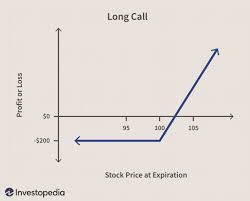
\includegraphics[width=0.4\textwidth]{graphics/LongCall.jpg}
%         }%
%         \subfigure[Short Call]{%
%           \label{fig:second}
%           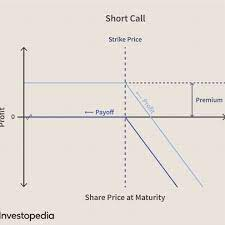
\includegraphics[width=0.4\textwidth]{graphics/ShortCall.jpg}
%         }\\ %  ------- End of the first row ----------------------%
%         \subfigure[Long Put]{%
%             \label{fig:third}
%             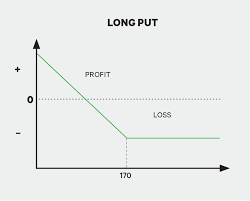
\includegraphics[width=0.4\textwidth]{graphics/LongPut.png}
%         }%
%         \subfigure[Short Put]{%
%             \label{fig:fourth}
%             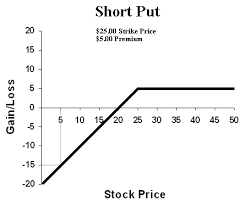
\includegraphics[width=0.4\textwidth]{graphics/ShortPut.png}
%         }%
%     \end{center}
%     \caption{Payoff Diagrams}
%     \label{fig:my_label}
% \end{figure}






\subsection{A Note on Volatility}
While it is impossible to predict the volatility over the duration of an option, we can use a few estimators to find \textbf{historical volatility}.
\\ 
Historical Volatility is defined as the standard deviation of the returns of the underlying multiplied by the square root of the number of time intervals. That is,
$$\sigma^{2}=\frac{1}{N-1}\sum_{n=1}^{N}(x_{i}-\overline{x})^{2}$$
\\
\begin{center}
    $\sigma$ - Volatility \\
    $N$ - Number of observations \\
    $x_{i}$ - Percent return on observation i \\
$\overline{x}$ - Mean return over N observations \\
\end{center}

We can then annualize this by multiplying $\sigma$ by $\sqrt{252}$, the number of trading days in a year.
\\
\\
Another common measure of volatility is \textbf{Yang-Zhang Volatility Model} \cite{YangZhang}. First derived in 2000, the model builds upon the  \textbf{Rogers-Satchell Volatility measure}\cite{RogersSatchell} from 1991 and takes into account opening jumps, drift and estimation error. This measure is often used in real applications since it converges to true historical volatility with much fewer observations than previous methods. \\
\\
As such, it can be thought of as the combination of the close-open volatility (overnight, open-close volatility, and a weighted average of the Rogers-Satchell Volatility
$$\sigma_{Yang-Zhang} = \sqrt{\sigma_o^2+k\sigma_c^2+(1-k)\sigma_{TS}^2}$$
Where 
$$k=\frac{\alpha - 1}{\alpha + \frac{T+1}{T-1}}$$

$$\sigma_o^2 = \frac{1}{T-1}\sum_{t=1}^T \left(\ln{\frac{o_t}{c_{t-1}}} - Avg\ln{\frac{o_t}{c_{t-1}}}\right)^2, overnight \; volatility$$

$$\sigma_c^2 = \frac{1}{T-1}\sum_{t=1}^T \left(\ln{\frac{c_t}{o_{t}}} - Avg\ln{\frac{c_t}{o_{t}}}\right)^2, open-close \; volatility$$

$$\sigma_{RS} = \sqrt{\frac{1}{T}\sum_{t=1}^{T}\ln\left(\frac{h_{t}}{c_{t}}\right)\ln\left(\frac{h_{t}}{o_{t}}\right)+\ln\left(\frac{l_{t}}{c_{t}}\right)\ln\left(\frac{l_{t}}{o_{t}}\right)}, Rogers-Satchell\ Volatility$$
\vspace{.5mm}
$$\alpha = \frac{E[(u(u-c)+d(d-c))^2]}{\sigma^4(1-f)^2}$$
$$T = number \; of \; days \; in \; the \; sample \; period$$
$$o_t = open \; price \; on \; day \; t$$
$$h_t = high \; price \; on \; day \; t$$
$$l_t = low \; price \; on \; day \; t$$
$$c_t = close \; price \; on \; day \; t$$




%\documentclass{article}
%\usepackage[utf8]{inputenc}
%\usepackage{graphicx}
%\usepackage{amsmath}
%\begin{document}

\section{Black Scholes Introduction}

\subsection{Brief History}
In 1973, Fischer Black and Myron Scholes published the Black-Scholes Model in an article named “The Pricing of Options and Corporate Liabilities.” Their objective was to create a riskless portfolio by buying and selling European options in just the “right way.”  Today, this model is a widely applied mathematical model in the modern financial world and it serves as the foundation for many investment banks and hedge fund strategies.

\subsection{Assumptions}
The Black-Scholes model assumes ideal market conditions. The model assumes short-term interest rates are constant, stocks pay no dividends, there are no transaction costs for stocks, one can borrow fractions of a stock, and short selling is allowed. The model also assumes the underlying stock price follows a geometric Brownian motion with constant volatility. Geometric Brownian motion is a continuous-time stochastic process where the random quantity follows an exponential trend with random drifts away from the trend. More precisely, the ratio between current and initial stock price follows a random log-normal distribution. The differential equation that models this behavior is the following:

\[ dS = \mu Sdt + \sigma Sdz\]


$$S - stock \;price$$
$$\mu - expected\;value\;of\;stock\;price$$
$$\sigma - standard\; deviation\; of\; stock\; price$$
$$t - time$$ 
$$z - standard\; Brownian\; Motion$$


\subsection{Input}
The Black-Scholes model takes into account five inputs: strike price, current stock price, days until expiration, risk-free rate or the interest rate on US Treasury Bonds, and the underlying stock's volatility. Moreover, the model only takes into account European Options exercised at the date of maturity. \cite{BS}

% \begin{itemize}
% \item Option - Contract giving the owner the right to buy or sell an underlying asset at a specific price and date
% \item Strike Price - price that a buyer assigns to an option upon purchase
% \item Expiration Time - Deadline one can call or sell a particular option by 
% \item Risk-free Interest Rate - The US Treasury Bill interest rate
% \item Volatility - fluctuation or randomness of stock price 
% \end{itemize}



\subsection{Derivation}
The Black-Scholes model is derived from a partial-differential equation. We will derive this model using Ito's Lemma and solve the partial differential equation for the model. First we have the stochastic process of an underlying stock modelled using the Geometric Brownian Motion \cite{BSDerivation}:

\[ \frac{dS}{S} = \mu dt + \sigma dW\]


$$S - stock\; price$$
$$\mu - average\; growth\; rate\; of\; stock\; price$$
$$t - time$$
$$dW - sample\; from\; standard\; normal\; distribution$$
$$\sigma - standard\; deviation\; of\; stock\; price$$


Next, Ito's Process is a generalized Wiener's process modeled by the formula:

\[ S_t = S_0 + \int_{0}^{t}a_{s}ds + \int_{0}^{t}b_{s}dW_{s}\]


$$S_t - stock\; price\; at\; time\; t$$
$$S_0 - stock \;price\; at\; time\;0$$
$$a,b - parameter\; functions$$
$$ W - Wiener's\; process $$
$$\int_{0}^{t}a_{s}ds - interest\; over\; time\; [0,t]$$
$$\int_{0}^{t}b_{s}dW_{s} - randomness $$



After, we will differentiate this equation on both sides to obtain:

\[ dS_t = a_{t}dt + b_{t}dW_{t}\] such that $x_0 = x$

\vspace{.5mm}

Now, let's generalize the process such that $a,b$ could be a function of the stock price:

\[ dS_t = S +  a(S_t, t)dt + b(S_t, t)dW_t \]


Ito's lemma states that if $S_t$ is a Wiener's process and $G(S_t, t)$ is a function of $S_t$ then $G$ also follows the Wiener's process in this form:

\[ dG = \left(\frac{\partial G}{\partial x}a + \frac{\partial G}{\partial t} + \frac{1}{2}\frac{\partial^2G}{\partial x^2}b^2\right)dt + \frac{\partial G}{\partial x}bdz\]

Using the geometric Brownian motion formula, we can find $G(x_t, t)$ for $a = \mu S$ and $b = \sigma S$ where in this case, $G$ will be substituted by $V$, the value of the option.

\[ dV = \left(\frac{dV}{dS}\mu S + \frac{dV}{dS} + \frac{1}{2}\frac{d^2V}{dS^2}\sigma^2S^2\right)dt + \frac{dV}{dS}\sigma SdW\]


The riskless aspect of Black-Scholes is derived from the concept of a delta hedged portfolio. A delta hedged portfolio allows the holder to reap short term benefits while holding a long term position in the stock market. This is achieved by outing portions of a long term position to hedge losses made by short term positions. The delta hedge portfolio is described using the formula: 

\[\Pi = -V + \int \frac{dV}{ds}ds\] where $\Pi$ is the value of the portfolio and $V$ is the value of the option.  

Now, the profit and loss of the value of the option over time period [$t$, $t + \Delta t$] is

\[ \Delta \Pi = -\Delta V + \frac{dV}{dS}\Delta S \] 

Let us discretize the Geometric Brownian motion and the valuation formula we derived using Ito's lemma: 

\[ \Delta S = Sv \Delta t + S\sigma \Delta W\]
\[ \Delta V = \left(\frac{\partial V}{\partial S}\mu S + \frac{\partial V}{\partial S} + \frac{1}{2}\frac{\partial^2V}{\partial S^2}\sigma^2S^2\right)\Delta t + \frac{\partial V}{\partial S}\sigma S \Delta W\]

Substitute these discretized equations into the profit-and-loss delta hedge equation: 

\[ \Delta \Pi = \left(- \frac{\partial V}{dt} - \frac{1}{2} \sigma^2 s^2 \frac{\partial^2V}{\partial S^2}\right)\Delta t\]

Notice how $\Delta W$, the uncertainty, has been eliminated from the equation. The portfolio is effectively 'riskless' now. Thus, the rate of return of this portfolio must equal to any other riskless instrument. This can be shown in the following model:

\[ r \Pi \Delta t = \Delta \Pi \] where r is the annual riskless interest rate 

Substituting $\Pi$ and $\Delta \Pi$, we have 

\[ r\left(-V + S\frac{dV}{dS}\right)\Delta t = \left(- \frac{dV}{dt} - \frac{1}{2} \sigma^2 s^2 \frac{d^2V}{dS^2}\right)\Delta t\]


Simply the equation above and we arrive at the Black-Scholes PDE: 

\begin{equation}
	\frac{\partial \mathrm V}{ \partial \mathrm t } + \frac{1}{2}\sigma^{2} \mathrm S^{2} \frac{\partial^{2} \mathrm V}{\partial \mathrm V^2}
	+ \mathrm r \mathrm S \frac{\partial \mathrm V}{\partial \mathrm S}\ -
	\mathrm r \mathrm V = 0 
\end{equation}

To solve the PDE, recall its boundary conditions:
\[C(0,t) = 0\: for\: all\: t\]
\[C(S,t) ~ S-Ke^{-r(T-t)} \:as\: S\rightarrow\infty\]
\[C(S,T) = max\{S-K,0\}\]
The first two conditions are possible as \textit{S} goes to 0 or infinity, and the last condition computes the value of the option at the time it matures. 
\newline
The PDE is a Cauchy-Euler equation, and can be transformed into a diffusion equation when we do change-of-variable.
\[\tau = T-t\]
\[u=Ce^{r\tau}\]
\[x=\ln\left(\frac{S}{K}\right)+(r-\frac{1}{2}\sigma^2)\tau\]
Then the PDE turns into a diffusion equation:
\[\frac{\partial u}{\partial \tau} = \frac{\partial^2u}{\partial x^2}\]
And the terminal condition 
\[C(S,T)=max\{S-K,0\}\] is now
\[u(x,0)=u_0(x):=K(e^{max\{x,0\}}-1)=K(e^x-1)H(x)\]
where $H(x)$ is the Heaviside step function, which corresponds to enforcement of the boundary data when $t=T$.
Using the convolution method to solve the diffusion equation, we have
\[u(x,\tau) = \frac{1}{\sigma\sqrt{2\pi\tau}} \int_{-\infty}^{\infty}u_0(y)\exp\left[-\frac{(x-y)^2}{2\sigma^2\tau}\right]dy\]
which simplifies to 
\[u(x,\tau)=Ke^{x+\frac{1}{2}\sigma^2\tau}N(d_1)-KN(d_2)\]

where $N(\cdot)$ is the standard normal cumulative distribution function,
\[d_1 = \frac{1}{\sigma\sqrt{\tau}}\left[\left(x+\frac{1}{2}\sigma^2\tau\right)+\frac{1}{2}\sigma^2\tau\right]\]
\[d_2 = \frac{1}{\sigma\sqrt{\tau}}\left[\left(x+\frac{1}{2}\sigma^2\tau\right)-\frac{1}{2}\sigma^2\tau\right]\]

Reverting back to the original variables, substituting $X$ for $K$, we can derive the call and put function.
\\

The Black-Scholes call formula:
\[C(S,t) = SN(d_1) - Xe^{-r(T-t)}N(d_2)\]



The Black-Scholes put formula:
\[P(S,t) = Xe^{-r(T-t)}N(-d_2)-SN(-d_1)\]


\subsection{The Model}

\begin{align*}
C_{call} &= SN(d_1) - Xe^{-rT}N(d_2) \\
P_{put} &= Xe^{-rT}N(-d_2) - SN(-d_1) \\ 
d_1 &= \frac{log(S/X) + (r + \frac{\sigma^2}{2})}{\sigma\sqrt{T}} \\
d_2 &= d_1 - \sigma\sqrt{T}
\end{align*}


$$C_{call} - call\; price$$
$$P_{put} - put\; price$$
$$S - current\; option\; price\; of \;stock $$
$$X - strike\; price\; of\; stock$$ 
$$r - annual\; risk-free\; interest\; rate$$
$$T - time\; left\; until\; expiration (yr)$$
$$\sigma - annualized\; volatility\; of\; stock$$ 
$$N - standard\; normal\; cumulative\; distribution\; function$$





% \subsection{Black-Scholes Simulation}

% To determine the fair option price from the Black-Scholes model for put and call options, we calculate the factors $d_1$ and $d_2$ using the general Black Scholes formula derived above. \\

% We then simulate this model across the AAPL option dataset, isloating for moneyness and time until expiry. used for all three models and determine the Root Squared Mean Error (RSME) in terms of USD of the project option price. The RSME must be differentiated between intervals of moneyness, time intervals,and volume type because each interval might have different dynamics when it comes to pricing. 


% This code will output the BS RSME for the AAPL stock based on the mentioned intervals and volume types. 
% This is not useful either

% \section{Results \& Analysis}

% The RSME for the fair option price projected by the BS model has been categorized by volume type, moneyness, and time. The output of the simulated program is shown in the figure above and it has been categorized accordingly. The results showed that the RSME ranges from approximately 0.28 USD to 1.13 USD. This shows that the BS model was fairly accurate since AAPL option prices range from 80 to 200. 

% This is innacurate. We will put discussion in conclusion




%\end{document}
\section{Monte Carlo Simulation Introduction}
A Monte Carlo Simulation is a mathematical technique that enables us to take risk into account when faced with uncertainty. The model is used in situations with stochastic outcomes and the result is a probability distribution, providing decision-makers with a range of possibilities, and the likelihood of occurrence for every course of action. The model has a wide range of applications in the real-world, mainly in fields involving a large number of random factors where predicting future outcomes becomes highly complex, such as finance and engineering. \cite{MCDS}

We use a Monte Carlo Simulation to model the movement of a stock. Some considerations when building this model include:
\begin{itemize}
\item  The ending price of the stock. 
\item  External factors such as volatility and interest rates.
\item  Geometric Brownian Motion model. This model assumes changes in stock prices/returns are independent and thus cannot use past events to predict the future, which we then by run many times using the inputs and provide a distribution of results.
\end{itemize}
Some limitations to this model include the tedious and time consuming implementation which requires thousands of iterations. Additionally, like any other mathematical model used to simulate the real world, assumptions have to be made in order to simplify reality. For example, most Monte Carlo Simulations used to predict the return of a stock assume that returns are normally distributed.
\\
We use a Monte Carlo Simulation to simulate stock movements, which will give us the expected payoff of a call option. 


\subsection{Derivation}
To begin, the Geometric Brownian Motion model was used to generate many possible future stock prices using the following stochastic differential equation\cite{MCS}:

\begin{equation}
   \frac{dS_{t}}{S_{t}} = \mu dt + \sigma dW_{t}
\end{equation}
where:

$$S_{t} - represents\; the\; price\; of\; the\; stock\; at\; any\; time\; t$$
$$\mu - drift$$
$$\sigma - volatility$$
$$W_{t} - Brownian\; motion\; (stochastic\; term)$$
$$dS_{t} - change\; in\; price\; of \;the \;stock\; over\; time$$
$$dt - change \;in \;time$$

 
We can integrate equation (2) to obtain:
\begin{equation}
   S_{T} = S_{t}+ r(T-t) + \sigma (W_{T}-W_{t})
\end{equation}
 
 where:
 \begin{equation} 
 W_{T}-W_{t} \sim \mathcal{N}(0,T-t)
 \end{equation}
 
 This tells us that the term $\sigma dW_{t}$ is normally distributed with mean \textit{0}, variance "$T-t$ and a non-zero standard deviation. 
 
\paragraph{}
 
Brownian Motion follows both the Markov and Martingale property. The Markov  theorem (Memorylessness) explains how the value of a stochastic process in the future only depends on the current value, whereas the Martingale explains how the conditional expectation of the value depends on the present value, provided information about historical values. Using Geometric Brownian Motion, the future price of the stock will be log normally distributed. 
\paragraph{}
 
The solution to equation (2) can be achieved using Ito's lemma, which leads to:
 
\begin{equation}
    \ln{S_{t} = \ln{S_{o} + \left(\mu - \frac{1}{2}\sigma^2\right)dt+\sigma dW_{t}}}
\end{equation}
  Which simplifies to:
  \begin{equation}
    S_{t} = S_{o}e^{\left(\mu - \frac{1}{2}\sigma^2\right)dt+\sigma dW_{t}}
  \end{equation}
 
 where $S_{o}$ is the initial stock price.

 \paragraph{}
 Next, these parameters will be assigned values including the initial price, total time, change in time, drift term and the volatility value. The volatility was found using historical and Yang-Zhang volatility, whereas the average historical return was used to find the drift.  Repeated use of this formula can then be used to generate a significant number of stochastic price paths between current and expiration date.
 
  \paragraph{}
  
Once the price paths have been simulated, we take the expected extrinsic value of the option, which will be the fair value of the option. From the derivation of the Black-Scholes Formula, a Monte Carlo simulation should converge to the price given by Black-Scholes formula for a large number of trials.





\section{Machine Learning Model Introduction}
In our project, we will use a Multi-layer Perceptron Neural Network to price an option. 
\subsection{Neural Network}
At their core, neural networks work by imitating the neurons in our brains to try and make predictions or classifications. The most popular neural network used to predict numerical data is a multi-layer perceptron (MLP) which works by receiving independent input into a few nodes, passing the data through a series of hidden layers of neurons, and predicting an output. Based on the accuracy of the output, the weight given to each neuron changes and the model runs again until it reaches an optimal value. 

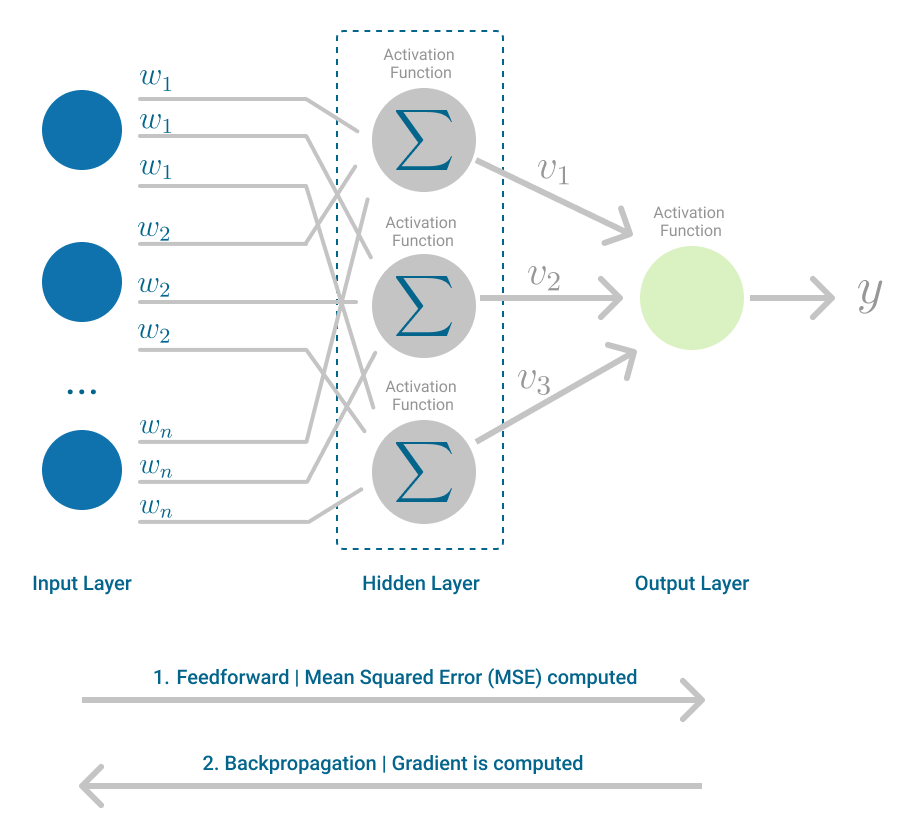
\includegraphics[width=.5\textwidth]{graphics/MLNNGraphic.png}
\\
As can be seen from the above image, the model works by taking a set of numerical inputs, multiplying each by a weight which is then passed through a nonlinear activation function in the first hidden layer. Note that if the activation function is linear, this MLP would work like a multiple linear regression or logistic regression. These activation functions then run and take on weights of their own, which then get passed on to other hidden layers. Once the output is calculated, it is compared to the expected output and the weights are tuned to minimize the model’s loss function or the distance between the model's output and the expected output. This optimization happens through gradient descent or an improved version of it. After the MLP has trained for enough time, it converges to a local minimum, and the model is considered trained. MLP models have been extensively used to model financial data and make predictions based on numerical values. We use a stock option’s strike price, current price, time until expiration, interest rate, and historical volatility in order to predict the best value for the stock option. \cite{MLIntro}

\subsection{Root Mean Squared Error}
Root Mean Squared Error (RMSE) is calculated to be the standard deviation of the prediction errors (otherwise known as \textit{residuals}. It can be more specifically described as the square root of the mean of the square of the errors. In machine learning, RMSE is used to measure how accurate the set of predictions from a model is. \cite{RMSE}
$$RMSE = \sqrt{\frac{1}{n}\sum_{i=1}^n S_i - {O_i}^2}$$
Where 
$$n = number\; of \; observations$$
$${O_i}^2 = observed\; value$$
$$S_i = predicted \; values$$
% \subsection{Yang-Zhang Volatility Model}

\section{Procedure}
\subsection{Data}
We downloaded and imported one year of Apple Inc.'s option data as our dataset and cleaned the data by removing null values. We then pulled three month treasury rates as well as the underlying stock's data. With this, we populated each row of our data with the risk-free rate as well as the 15, 30, and 60 day volatilities and the 30-day-lookback Yang-Zhang volatility\cite{underlying}. As our output variable, we tried to estimate the midpoint of the bid-ask spread on each option as the fair market price of the option.
\\ \\
In order to isolate for different option dynamics, we also filtered the data into three levels of moneyness, 
\begin{enumerate}
    \item $0.2 < \frac{S}{K} < 0.8 $ (Deep Out the Money)
    \item $0.8 < \frac{S}{K} < 1.2 $ (At the Money)
    \item $1.2 < \frac{S}{K} < 1.8 $ (Deep In the Money)
\end{enumerate}
and three levels of time until expiry
\begin{enumerate}
    \item $0 < T < 30 $
    \item $30 < T < 90 $
    \item $90 < T < 300 $
\end{enumerate}


\subsection{Black-Scholes}
For each row of the data, we ran the Black-Scholes formula with a different volatility model and compared it with the midpoint of the bid/ask spread. From that, we found and tabulated the root mean squared error.

\subsection{Monte Carlo}
As we did with Black-Scholes, we ran the Monte Carlo simulation by generating 2000 paths the stock could take until expiry and finding the option's extrinsic value on each one. By taking the expected value of these results, we found the fair price of the option and compared it to the bid/ask midpoint. 

\subsection{MLP}
For our MLP model, we performed a 80-20 train-test split on our normalized data and trained the model until convergence. We then predicted values for our testing data and found the root mean squared error of our predictions.

\section{Discussion}
Throughout all 3 models, we can say that further dated options are less accurate. The Root Mean Squared Error (RMSE) for the 90-300 days till expiry options are significantly higher than the other two tested time periods. 

We see that the MLP model is the most accurate because the RMSE is consistently lower across all 3 time periods and moneyness options tested. 

Based on our results, we see that the further dated options were also less accurate. This is what we expect for two reasons:
\begin{enumerate}
    \item We used the 3 month Treasury interest rate.
    \item Far dated options (90-300 DTE) are more difficult to model and have more variability.
\end{enumerate}

At the Money (ATM) options were the least accurate when compared to In the Money (ITM) and Out the Money (OTM). We believe this happens for two reasons:
\begin{enumerate}
    \item They have the greatest sample size, meaning that more variability can occur in the option pricing. 
    \item These options are the most sensitive to price movements. A small move in price, either up or down, can mean they expire worthless.
\end{enumerate}
\subsection{Most Accurate Model}
MLP is the most accurate because the RMSE is the least consistently, across the OTM, ATM, ITM options, and also for the 3 tested time periods. We believe that using the Yang-Zhang Volatility model, one of the most accurate volatility models used by quant firms to account for overnight jumps and a recent advancement in volatility models, in cumulation with a neural network allowed the option pricing data to be trained and tested accurately alongside the historical AAPL options data. Before we ran the models, we hypothesized that the MLP would be the most accurate model as the metrics behind the testing are more extensive compared to the Black-Scholes and Monte Carlo Simulations. 
 
\section{Conclusion}
Our goal was to to simulate a model which predicts the price of a European Call option.  We derived the Black-Scholes Partial Differential Equation, solve it into an equation to price call options, and simulate the model using Python. We also explored the use of the Monte Carlo Simulation using python and applied it to our model. In addition, we also used a Multi-layer Perceptron Neural Network and compared it with the other two models. There are some limitations to our research. Like any mathematical model used to simulate the real world, assumptions had to be made in order to simplify the complex reality of the stock market. An example of an assumption we made for the Black-Scholes Model is that we assumed short term interest rates were constant and that the stock paid no dividends. Another assumption we made in the Monte Carlo Model was that the returns of the stock were log-normally distributed. All these assumptions were made in the effort of making it possible to model the intricate nature of the financial world using mathematics and code. 

\appendix

\section{Black-Scholes}
\begin{center}
\begin{tabular}{c|c|c|c|c|c|c|c}
Moneyness & DTE & BS($\sigma_{15}$) & BS($\sigma_{30}$) & BS($\sigma_{60}$) & BS($\sigma_{YZ}$) & n \\
\hline
$0.2 < \frac{S}{K} < 0.8$ & 0-30 & 0.28406 & 0.2824 & 0.28208 & 0.28244 & 9923 \\
& 30-90 & 0.79928 & 0.78487 & 0.78157 & 0.78812 & 12749 \\
& 90-300 & 1.87818 & 1.85116 & 1.86817 & 1.85932 & 20594 \\
$0.8 < \frac{S}{K} < 1.2$ & 0-30 & 0.55362 & 0.49284 & 0.49463 & 0.5436 & 39587 \\
& 30-90 & 1.12992 & 0.92483 & 0.92757 & 1.05482 & 22312 \\
& 90-300 & 2.42869 & 2.2095 & 2.39884 & 2.30437 & 12859 \\
$1.2 < \frac{S}{K} < 1.8$ & 0-30 & 0.08636 & 0.08536 & 0.08572 & 0.08611 & 8965 \\
& 30-90 & 0.27744 & 0.22102 & 0.2168 & 0.2307 & 8258 \\
& 90-300 & 1.12154 & 0.84465 & 0.8831 & 0.8546 & 10809 \\
\end{tabular}
\end{center}

\section{Monte Carlo}
\begin{center}
\begin{tabular}{c|c|c|c|c|c|c}
Moneyness & DTE & MC($\sigma_{15}$) & MC($\sigma_{30}$) & MC($\sigma_{60}$) & MC($\sigma_{YZ}$) & n \\
\hline
$0.2 < \frac{S}{K} < 0.8$ & 0-30 & 0.32046 & 0.31858 & 0.31689 & 0.3236 & 9923 \\
& 30-90 & 0.74163 & 0.73044 & 0.72298 & 0.73785 & 12749 \\
& 90-300 & 1.57233 & 1.53581 & 1.56398 & 1.5501 & 20594 \\
$0.8 < \frac{S}{K} < 1.2$ & 0-30 & 0.55676 & 0.49552 & 0.49534 & 0.54542 & 39587 \\
& 30-90 & 1.10122 & 0.88674 & 0.88983 & 1.01515 & 22312 \\
& 90-300 & 2.25394 & 1.98149 & 2.13289 & 2.0574 & 12859 \\
$1.2 < \frac{S}{K} < 1.8$ & 0-30 & 0.08647 & 0.08613 & 0.08601 & 0.08654 & 8965 \\
& 30-90 & 0.2788 & 0.22379 & 0.21957 & 0.23073 & 8258 \\
& 90-300 & 1.09223 & 0.80456 & 0.83578 & 0.80953 & 10809 \\
\end{tabular} 
\end{center}

\section{MLP}
\begin{center}
\begin{tabular}{c|c|c|c}
Moneyness & DTE & MLP $(\sigma_{ALL})$ & n \\
\hline
$0.2 < \frac{S}{K} < 0.8$ & 0-30 & 0.16909 & 9923 \\
& 30-90 & 0.21028 & 12749 \\
& 90-300 & 0.40256 & 20594 \\
$0.8 < \frac{S}{K} < 1.2$ & 0-30 & 0.27738 & 39587 \\
& 30-90 & 0.33366 & 22312 \\
& 90-300 & 0.31624 & 12859 \\
$1.2 < \frac{S}{K} < 1.8$ & 0-30 & 0.05406 & 8965 \\
& 30-90 & 0.10596 & 8258 \\
& 90-300 & 0.1408 & 10809 \\
\end{tabular} 
\end{center}

\section{Terms}
DTE represents the Days Till Expiry. The ranges for the ratio of S to K are defined as: 
\begin{enumerate}
    \item Deep Out the Money: $0.2 < \frac{S}{K} < 0.8$
    \item At the Money: $0.8 < \frac{S}{K} < 1.2$
    \item Deep In the Money: $1.2 < \frac{S}{K} < 1.8$
\end{enumerate}
% \begin{left}



% \begin{table}
% \centering
% \hskip-9.95705cm
% \begin{tabular}{llllll}
% Moneyness                             & Time Until Expiry & Monte Carlo(S15) & Monte Carlo(S30) & Monte Carlo(S60) & Monte Carlo(SYZ)  \\
% Deep in the money (0.2  s/k  0.8)     & 0-30              & 0.32046          & 0.31858          & 0.31689          & 0.3236            \\
%                                       & 30-90             & 0.74163          & 0.73044          & 0.72298          & 0.73785           \\
%                                       & 90-300            & 1.57233          & 1.53581          & 1.56398          & 1.5501            \\
% At the money (0.8  s/k  1.2)          & 0-30              & 0.55676          & 0.49552          & 0.49534          & 0.54542           \\
%                                       & 30-90             & 1.10122          & 0.88674          & 0.88983          & 1.01515           \\
%                                       & 90-300            & 2.25394          & 1.98149          & 2.13289          & 2.0574            \\
% Deep out of the money (1.2  s/k  1.8) & 0-30              & 0.08647          & 0.08613          & 0.08601          & 0.08654           \\
%                                       & 30-90             & 0.2788           & 0.22379          & 0.21957          & 0.23073           \\
%                                       & 90-300            & 1.09223          & 0.80456          & 0.83578          & 0.80953          
% \end{tabular}
% \end{table}


% \end{figure}


%\end{left}




%\bibliographystyle{plain} % We choose the "plain" reference style
\printbibliography

\end{document}
